\setcounter{chapter}{3}
\chapter{System Design and Architecture}
\label{ch:design}

\section{Architectural Overview}
\label{sec:arch-overview}

SmartHire follows a layered architecture comprising four tiers: a client-side presentation layer, an application logic layer, an AI services layer, and a data persistence layer. This separation allows each tier to evolve independently and simplifies testing. The presentation layer is a Next.js~15 single-page application that communicates with the backend through RESTful API routes. The application logic layer, also implemented within Next.js using its App Router API routes, handles request validation, business logic, and database interaction. The AI services layer wraps calls to Google's Gemini API for resume scoring and interview evaluation. The data persistence layer is a managed PostgreSQL instance on Supabase, organised into domain-specific schemas.

\begin{figure}[htbp]
\centering
\resizebox{0.95\textwidth}{!}{
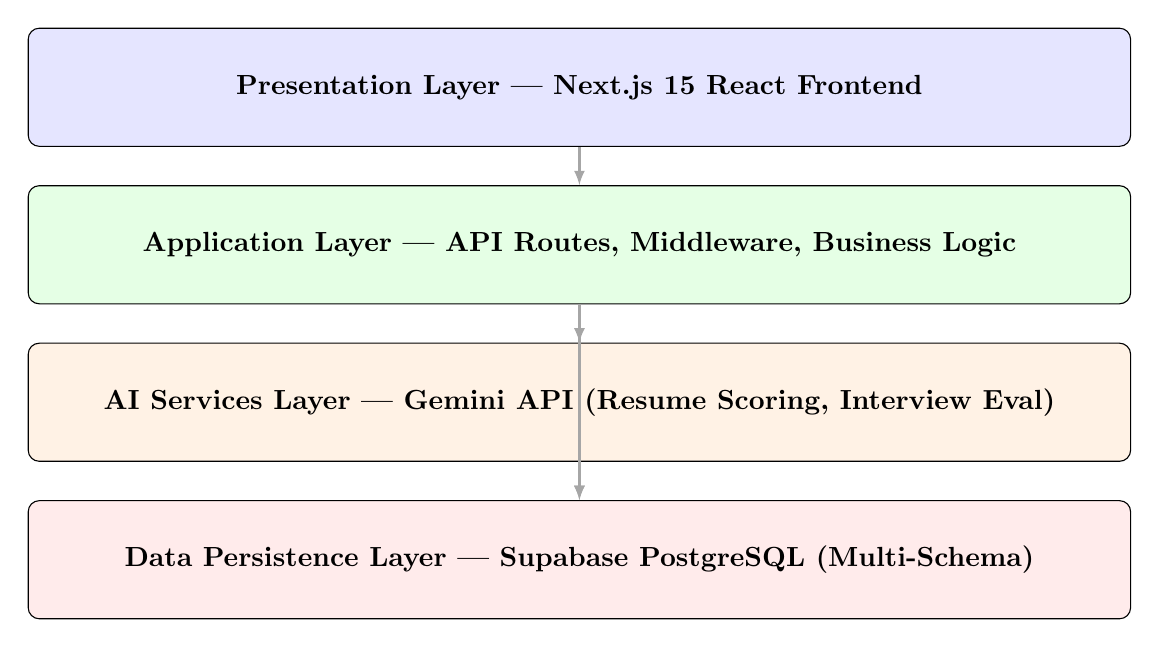
\begin{tikzpicture}[
  tier/.style={rectangle, draw, rounded corners, fill=#1, minimum width=14cm, minimum height=1.5cm, text centered, font=\bfseries},
  arrow/.style={-latex, thick, draw=gray!70}
]
  \node[tier=blue!10]   (pres) at (0,6)  {Presentation Layer --- Next.js 15 React Frontend};
  \node[tier=green!10]  (app)  at (0,4)  {Application Layer --- API Routes, Middleware, Business Logic};
  \node[tier=orange!10] (ai)   at (0,2)  {AI Services Layer --- Gemini API (Resume Scoring, Interview Eval)};
  \node[tier=red!8]     (data) at (0,0)  {Data Persistence Layer --- Supabase PostgreSQL (Multi-Schema)};

  \draw[arrow] (pres) -- (app);
  \draw[arrow] (app) -- (ai);
  \draw[arrow] (app) -- (data);
  \draw[arrow] (ai) -- (data);
\end{tikzpicture}
}
\caption{Four-tier layered architecture of SmartHire}
\label{fig:layered-arch}
\end{figure}

Figure~\ref{fig:layered-arch} illustrates the four tiers and their communication paths. The presentation layer issues HTTP requests to the application layer. The application layer may, depending on the endpoint, invoke the AI services layer (for operations requiring Gemini evaluation) or interact directly with the database. The AI services layer also reads from and writes to the database---for example, storing computed ATS scores alongside the corresponding application record.

\section{High-Level System Architecture}
\label{sec:highlevel}

\begin{figure}[htbp]
\centering
\resizebox{0.95\textwidth}{!}{
\begin{tikzpicture}[node distance=1.4cm, auto,
  comp/.style={rectangle, draw, rounded corners, fill=blue!8, text width=9em, text centered, minimum height=2.5em, font=\small},
  db/.style={cylinder, draw, shape border rotate=90, fill=red!8, minimum height=2em, minimum width=3em, aspect=0.3, font=\small},
  ext/.style={rectangle, draw, rounded corners, fill=orange!10, text width=8em, text centered, minimum height=2.2em, font=\small},
  arrow/.style={-latex, thick}
]
  \node[comp] (candidateUI) {Candidate Portal\\(React)};
  \node[comp, right=2.5cm of candidateUI] (recruiterUI) {Recruiter Portal\\(React)};
  \node[comp, right=2.5cm of recruiterUI] (adminUI) {Admin Dashboard\\(React)};

  \node[comp, below=1.8cm of recruiterUI] (apiLayer) {Next.js API Routes\\Middleware};

  \node[ext, below left=1.8cm and 1cm of apiLayer]  (gemini) {Gemini AI API};
  \node[db,  below=1.8cm of apiLayer]                (db)     {Supabase\\PostgreSQL};
  \node[ext, below right=1.8cm and 1cm of apiLayer] (storage) {Supabase\\Storage};

  \draw[arrow] (candidateUI) -- (apiLayer);
  \draw[arrow] (recruiterUI) -- (apiLayer);
  \draw[arrow] (adminUI)     -- (apiLayer);
  \draw[arrow] (apiLayer)    -- (gemini);
  \draw[arrow] (apiLayer)    -- (db);
  \draw[arrow] (apiLayer)    -- (storage);
\end{tikzpicture}
}
\caption{High-level component architecture}
\label{fig:highlevel}
\end{figure}

The high-level architecture (Figure~\ref{fig:highlevel}) shows the three frontend portals connecting to a shared API layer. The API layer mediates all access to external services (Gemini API) and storage backends (PostgreSQL database and Supabase file storage). This design ensures that frontend components never interact with the database directly, centralising access control and validation logic in the API layer.

\section{Database Design}
\label{sec:db-design}

\subsection{Multi-Schema Organisation}

SmartHire's PostgreSQL database is divided into domain-specific schemas rather than placing all tables in a single \texttt{public} schema. This design decision offers three advantages: logical grouping of related entities, simplified access control policies, and reduced risk of naming collisions as the system grows.

\begin{figure}[htbp]
\centering
\resizebox{0.95\textwidth}{!}{
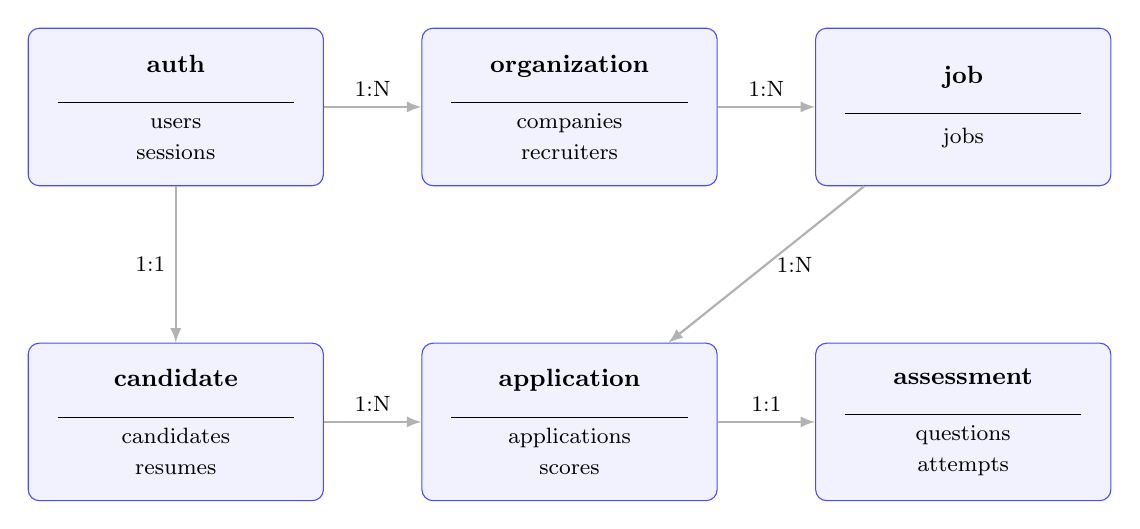
\begin{tikzpicture}[
  schema/.style={rectangle, draw=blue!70, fill=blue!5, rounded corners, text width=10em, text centered, minimum height=2cm, font=\small},
  arrow/.style={-latex, thick, draw=gray!60}
]
  \node[schema] (auth) at (0,4) {\textbf{auth}\\\rule{3cm}{0.3pt}\\\footnotesize users\\\footnotesize sessions};
  \node[schema] (org)  at (5,4) {\textbf{organization}\\\rule{3cm}{0.3pt}\\\footnotesize companies\\\footnotesize recruiters};
  \node[schema] (job)  at (10,4) {\textbf{job}\\\rule{3cm}{0.3pt}\\\footnotesize jobs};
  \node[schema] (cand) at (0,0) {\textbf{candidate}\\\rule{3cm}{0.3pt}\\\footnotesize candidates\\\footnotesize resumes};
  \node[schema] (app)  at (5,0) {\textbf{application}\\\rule{3cm}{0.3pt}\\\footnotesize applications\\\footnotesize scores};
  \node[schema] (assess) at (10,0) {\textbf{assessment}\\\rule{3cm}{0.3pt}\\\footnotesize questions\\\footnotesize attempts};

  \draw[arrow] (auth) -- (org) node[midway, above, font=\footnotesize] {1:N};
  \draw[arrow] (org)  -- (job) node[midway, above, font=\footnotesize] {1:N};
  \draw[arrow] (auth) -- (cand) node[midway, left, font=\footnotesize] {1:1};
  \draw[arrow] (job)  -- (app) node[midway, right, font=\footnotesize] {1:N};
  \draw[arrow] (cand) -- (app) node[midway, above, font=\footnotesize] {1:N};
  \draw[arrow] (app) -- (assess) node[midway, above, font=\footnotesize] {1:1};
\end{tikzpicture}
}
\caption{Multi-schema database organisation with entity relationships}
\label{fig:schema}
\end{figure}

\subsection{Entity Descriptions}

Table~\ref{tab:entities} summarises the principal database entities and their key attributes.

\begin{table}[htbp]
\centering
\caption{Principal database entities}
\label{tab:entities}
\small
\begin{tabular}{p{1.2in}p{1in}p{3.3in}}
\toprule
\textbf{Schema} & \textbf{Table} & \textbf{Key Attributes} \\
\midrule
\texttt{auth}        & \texttt{users}        & id, email, encrypted\_password, role, created\_at \\
\texttt{organization}& \texttt{companies}    & id, name, industry, website, logo\_url \\
\texttt{organization}& \texttt{recruiters}   & id, user\_id (FK), company\_id (FK), position \\
\texttt{job}         & \texttt{jobs}         & id, recruiter\_id (FK), title, description, skills[], status, location, salary\_range \\
\texttt{candidate}   & \texttt{candidates}   & id, user\_id (FK), phone, skills[], experience\_years \\
\texttt{candidate}   & \texttt{resumes}      & id, candidate\_id (FK), file\_url, parsed\_text, parsed\_at \\
\texttt{application} & \texttt{applications} & id, job\_id (FK), candidate\_id (FK), stage, ats\_score, mcq\_score, coding\_score, interview\_score, status \\
\texttt{assessment}  & \texttt{questions}    & id, job\_id (FK), type (mcq/coding), content, options[], correct\_answer, difficulty \\
\texttt{assessment}  & \texttt{attempts}     & id, application\_id (FK), question\_id (FK), answer, is\_correct, score, submitted\_at \\
\bottomrule
\end{tabular}
\end{table}

\subsection{Entity-Relationship Diagram}

Figure~\ref{fig:er} presents the complete ER diagram for the database, showing primary keys, foreign keys, and cardinality.

\begin{figure}[htbp]
\centering
\resizebox{0.95\textwidth}{!}{
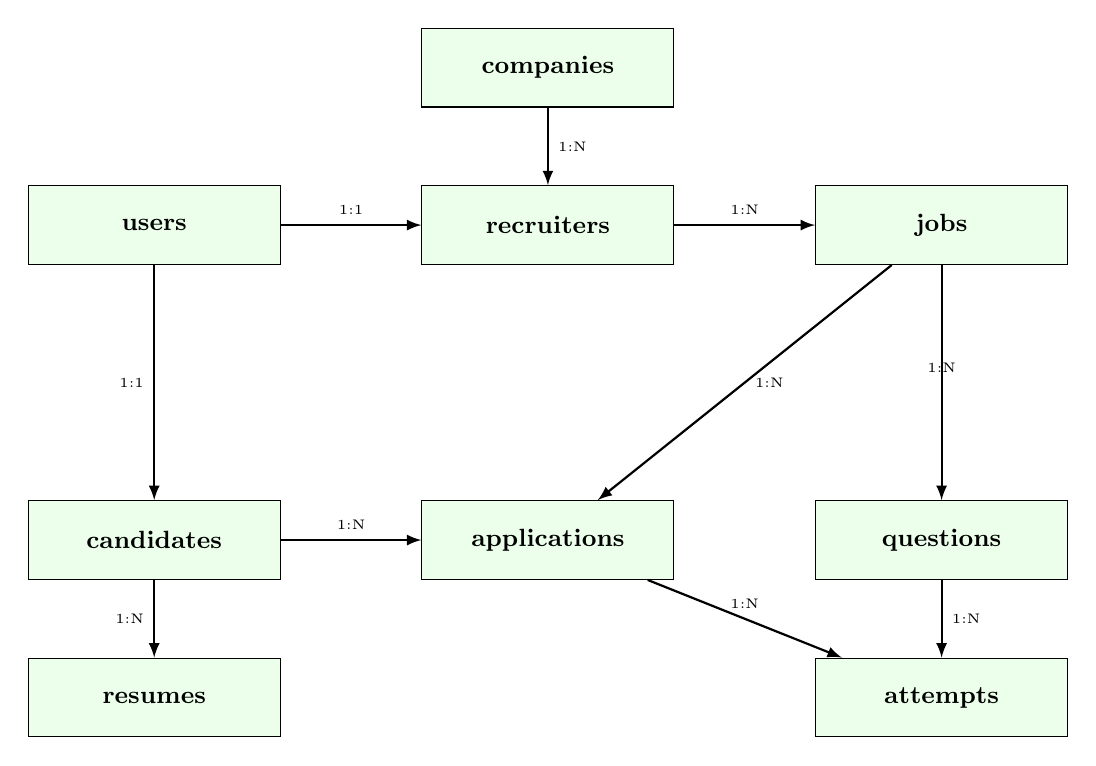
\begin{tikzpicture}[
  entity/.style={rectangle, draw, fill=green!8, minimum width=3.2cm, minimum height=1cm, font=\small\bfseries},
  rel/.style={diamond, draw, fill=yellow!15, minimum width=1.5cm, aspect=2, font=\footnotesize},
  arrow/.style={-latex, thick}
]
  \node[entity] (user) at (0,6) {users};
  \node[entity] (company) at (5,8) {companies};
  \node[entity] (recruiter) at (5,6) {recruiters};
  \node[entity] (job) at (10,6) {jobs};
  \node[entity] (candidate) at (0,2) {candidates};
  \node[entity] (resume) at (0,0) {resumes};
  \node[entity] (application) at (5,2) {applications};
  \node[entity] (question) at (10,2) {questions};
  \node[entity] (attempt) at (10,0) {attempts};

  \draw[arrow] (user) -- (recruiter) node[midway,above,font=\tiny]{1:1};
  \draw[arrow] (company) -- (recruiter) node[midway,right,font=\tiny]{1:N};
  \draw[arrow] (recruiter) -- (job) node[midway,above,font=\tiny]{1:N};
  \draw[arrow] (user) -- (candidate) node[midway,left,font=\tiny]{1:1};
  \draw[arrow] (candidate) -- (resume) node[midway,left,font=\tiny]{1:N};
  \draw[arrow] (candidate) -- (application) node[midway,above,font=\tiny]{1:N};
  \draw[arrow] (job) -- (application) node[midway,right,font=\tiny]{1:N};
  \draw[arrow] (job) -- (question) node[midway,above,font=\tiny]{1:N};
  \draw[arrow] (application) -- (attempt) node[midway,above,font=\tiny]{1:N};
  \draw[arrow] (question) -- (attempt) node[midway,right,font=\tiny]{1:N};
\end{tikzpicture}
}
\caption{Entity-Relationship diagram}
\label{fig:er}
\end{figure}

\section{Data Flow Diagrams}
\label{sec:dfd}

\subsection{DFD Level 0 --- Context Diagram}

The context diagram (Figure~\ref{fig:dfd0}) represents SmartHire as a single process interacting with three external entities: Candidate, Recruiter, and the Gemini AI service.

\begin{figure}[htbp]
\centering
\resizebox{0.95\textwidth}{!}{
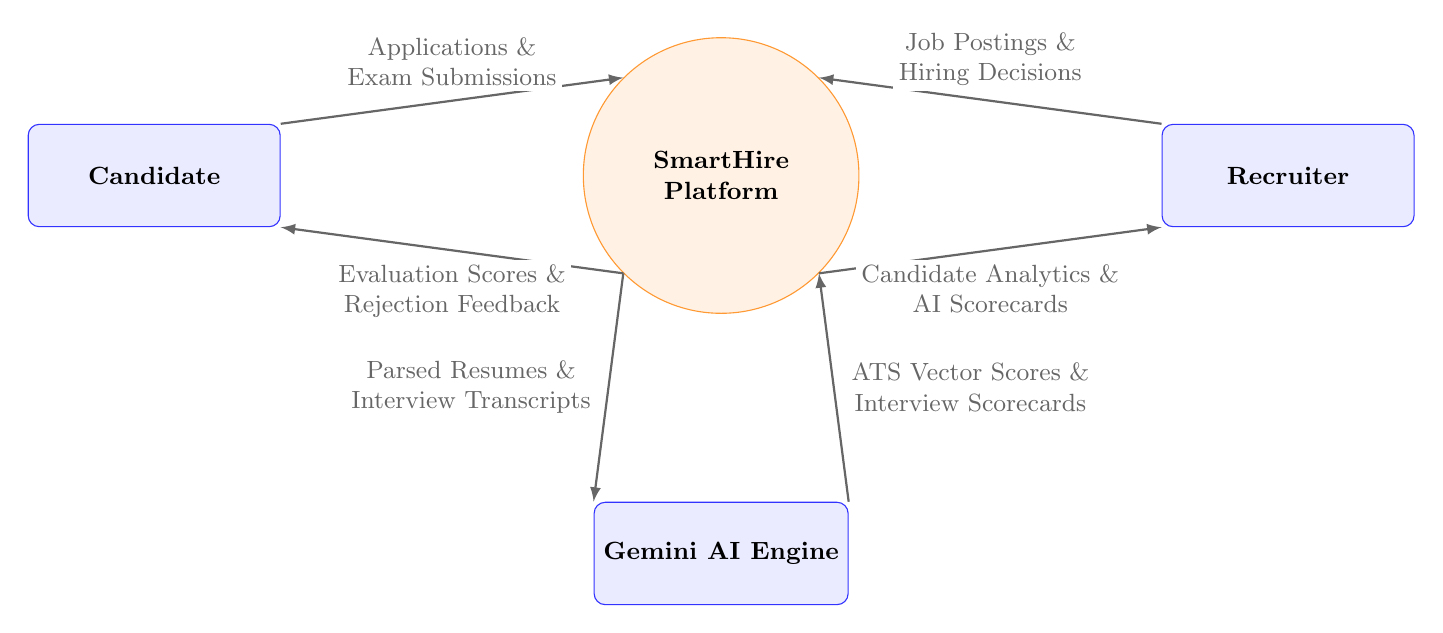
\begin{tikzpicture}[
  ext/.style={rectangle, draw=blue!80, fill=blue!8, minimum width=3.2cm, minimum height=1.3cm, rounded corners, font=\small\bfseries, align=center},
  process/.style={circle, draw=orange!80, fill=orange!10, minimum size=3.5cm, font=\small\bfseries, text width=2.8cm, align=center},
  arrow/.style={-latex, thick, color=gray!80!black},
  lbl/.style={font=\small, align=center, fill=white, inner sep=2pt}
]
  \node[ext] (cand) at (-7.2, 0) {Candidate};
  \node[process] (sys) at (0, 0) {SmartHire\\Platform};
  \node[ext] (rec) at (7.2, 0) {Recruiter};
  \node[ext] (ai) at (0, -4.8) {Gemini AI Engine};

  % Candidate <-> System
  \draw[arrow] (cand.north east) -- (sys.north west) node[midway, above=3pt, lbl] {Applications \&\\Exam Submissions};
  \draw[arrow] (sys.south west) -- (cand.south east) node[midway, below=3pt, lbl] {Evaluation Scores \&\\Rejection Feedback};

  % Recruiter <-> System
  \draw[arrow] (rec.north west) -- (sys.north east) node[midway, above=3pt, lbl] {Job Postings \&\\Hiring Decisions};
  \draw[arrow] (sys.south east) -- (rec.south west) node[midway, below=3pt, lbl] {Candidate Analytics \&\\AI Scorecards};

  % System <-> Gemini AI
  \draw[arrow] (sys.south west) -- (ai.north west) node[midway, left=4pt, lbl] {Parsed Resumes \&\\Interview Transcripts};
  \draw[arrow] (ai.north east) -- (sys.south east) node[midway, right=4pt, lbl] {ATS Vector Scores \&\\Interview Scorecards};
\end{tikzpicture}
}
\caption{DFD Level 0 --- Context diagram}
\label{fig:dfd0}
\end{figure}

\subsection{DFD Level 1}

Figure~\ref{fig:dfd1} decomposes the system into its six principal processing modules, showing data flows between them and the data stores.

\begin{figure}[htbp]
\centering
\resizebox{0.95\textwidth}{!}{
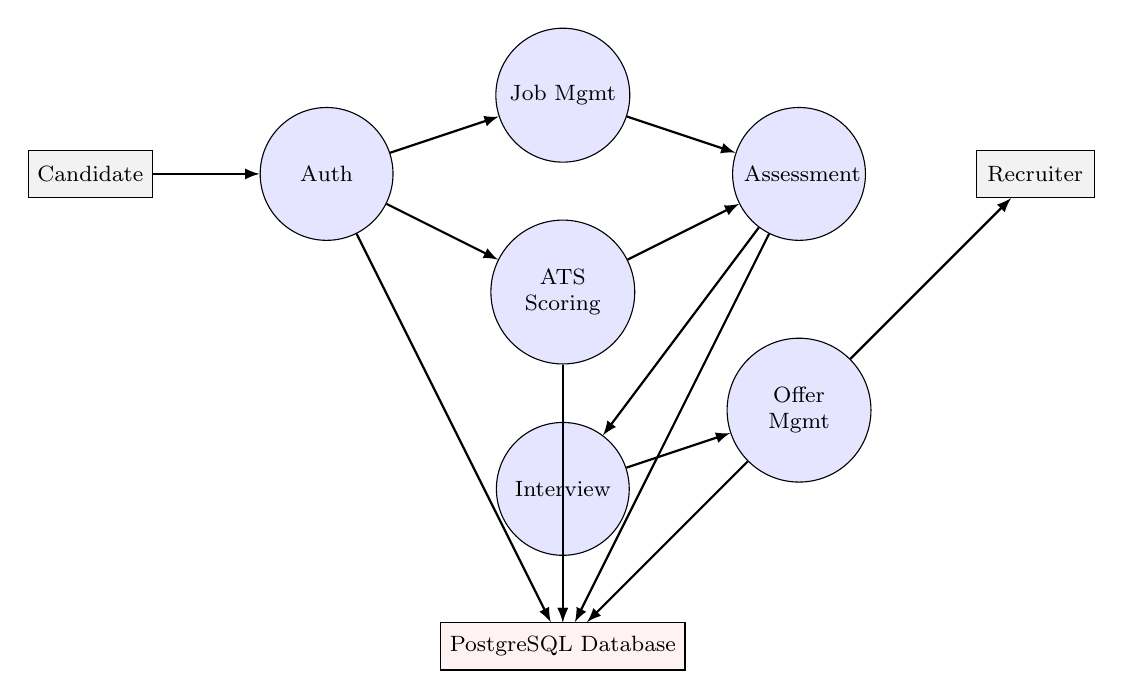
\begin{tikzpicture}[
  process/.style={circle, draw, fill=blue!10, minimum size=1.4cm, font=\footnotesize, text width=1.4cm, align=center},
  store/.style={rectangle, draw, fill=red!5, minimum width=2cm, minimum height=0.6cm, font=\footnotesize},
  ext/.style={rectangle, draw, fill=gray!10, minimum width=1.5cm, minimum height=0.6cm, font=\footnotesize},
  arrow/.style={-latex, thick, font=\tiny}
]
  \node[ext] (cand) at (-4,3) {Candidate};
  \node[ext] (rec)  at (8,3) {Recruiter};

  \node[process] (p1) at (-1,3) {Auth};
  \node[process] (p2) at (2,4) {Job Mgmt};
  \node[process] (p3) at (2,1.5) {ATS Scoring};
  \node[process] (p4) at (5,3) {Assessment};
  \node[process] (p5) at (2,-1) {Interview};
  \node[process] (p6) at (5,0) {Offer Mgmt};

  \node[store] (db) at (2,-3) {PostgreSQL Database};

  \draw[arrow] (cand) -- (p1);
  \draw[arrow] (p1) -- (p2);
  \draw[arrow] (p1) -- (p3);
  \draw[arrow] (p2) -- (p4);
  \draw[arrow] (p3) -- (p4);
  \draw[arrow] (p4) -- (p5);
  \draw[arrow] (p5) -- (p6);
  \draw[arrow] (p6) -- (rec);
  \draw[arrow] (p1) -- (db);
  \draw[arrow] (p3) -- (db);
  \draw[arrow] (p4) -- (db);
  \draw[arrow] (p5) -- (db);
  \draw[arrow] (p6) -- (db);
\end{tikzpicture}
}
\caption{DFD Level 1 --- Module decomposition}
\label{fig:dfd1}
\end{figure}

\section{Sequence Diagrams}
\label{sec:sequence}

\subsection{Candidate Application Flow}

The following sequence describes the interactions when a candidate applies for a job:

\begin{enumerate}[leftmargin=1.5em]
  \item Candidate uploads a PDF resume via the application form.
  \item The frontend sends a POST request to \texttt{/api/applications} with the resume file.
  \item The API route stores the resume in Supabase Storage and triggers the resume parsing service.
  \item The parsing service extracts text from the PDF, identifies skills and experience, and stores the parsed data.
  \item The ATS scoring module computes a relevance score by comparing parsed skills against the job's required skills.
  \item The computed score and parsed data are persisted in the \texttt{application.applications} table.
  \item A confirmation response is sent back to the candidate portal.
\end{enumerate}

\subsection{Recruiter Pipeline Management}

When a recruiter moves a candidate from one pipeline stage to another:

\begin{enumerate}[leftmargin=1.5em]
  \item The recruiter drags a candidate card on the Kanban board from the current stage column to the target stage column.
  \item The frontend issues a PATCH request to \texttt{/api/applications/\{id\}} with the new stage value.
  \item The API route validates that the transition is legal (stages can only advance forward, not backward) and updates the database.
  \item If the candidate is moved to a rejection stage, a rejection reason is recorded.
  \item The updated application state is returned to the frontend, and the Kanban board re-renders.
\end{enumerate}

\section{Authentication Workflow}
\label{sec:auth-workflow}

SmartHire delegates authentication to Supabase Auth, which provides JWT-based session management. Figure~\ref{fig:auth-flow} outlines the registration and login sequence.

\begin{figure}[htbp]
\centering
\resizebox{0.95\textwidth}{!}{
\begin{tikzpicture}[
  step/.style={rectangle, draw=blue!70, fill=blue!5, rounded corners, text width=9.0em, text centered, minimum height=2.8em, font=\small},
  decision/.style={diamond, draw=orange!80, fill=orange!10, text width=7.0em, text centered, aspect=2.2, font=\small},
  arrow/.style={-latex, thick, color=gray!80!black},
  lbl/.style={font=\small\bfseries, fill=white, inner sep=2pt}
]
  \node[step] (start) at (0,0) {User Login Request};
  \node[step] (submit) at (4.5,0) {Submit Credentials};
  \node[decision] (check) at (9.5,0) {Credentials Valid?};
  \node[step] (jwt) at (14.8,0) {Issue JWT Token};
  \node[step] (redirect) at (14.8,-2.8) {Redirect to Portal};
  \node[step] (error) at (9.5,-2.8) {Return Auth Error};

  \draw[arrow] (start) -- (submit);
  \draw[arrow] (submit) -- (check);
  \draw[arrow] (check) -- node[above=2pt, lbl]{Yes} (jwt);
  \draw[arrow] (check) -- node[right=4pt, lbl]{No} (error);
  \draw[arrow] (jwt) -- (redirect);
\end{tikzpicture}
}
\caption{Authentication workflow}
\label{fig:auth-flow}
\end{figure}

\section{ATS Resume Scoring Workflow}
\label{sec:ats-workflow}

The ATS scoring process operates in two phases: text extraction and relevance computation.

\textbf{Phase 1: Text Extraction.} When a candidate uploads a PDF resume, the system uses a text extraction library to convert the document into plain text. The extracted text is stored in the \texttt{candidate.resumes} table alongside the original file URL.

\textbf{Phase 2: Relevance Scoring.} The extracted resume text and the job description are sent to the Gemini API with a structured prompt requesting a relevance assessment. The API returns a composite score (0--10) along with dimensional breakdowns for skills match, experience relevance, and qualification alignment. These scores are recorded in the \texttt{application.applications} table.

\section{Coding Assessment Workflow}
\label{sec:coding-workflow}

\begin{figure}[htbp]
\centering
\resizebox{0.95\textwidth}{!}{
\begin{tikzpicture}[
  step/.style={rectangle, draw=teal!80, fill=teal!5, rounded corners, text width=9.5em, text centered, minimum height=2.5em, font=\small},
  arrow/.style={-latex, thick, color=gray!80!black}
]
  \node[step] (open) at (0,0) {Open Monaco IDE};
  \node[step] (editor) at (4.2,0) {Write Code Solution};
  \node[step] (submit) at (8.4,0) {Click Submit Solution};
  \node[step] (exec) at (8.4,-2.2) {Execute Against Test Cases};
  \node[step] (result) at (4.2,-2.2) {Evaluate Output Results};
  \node[step] (score) at (0,-2.2) {Record Score in DB};

  \draw[arrow] (open) -- (editor);
  \draw[arrow] (editor) -- (submit);
  \draw[arrow] (submit) -- (exec);
  \draw[arrow] (exec) -- (result);
  \draw[arrow] (result) -- (score);
\end{tikzpicture}
}
\caption{Coding assessment execution workflow}
\label{fig:coding-flow}
\end{figure}

The coding assessment module (Figure~\ref{fig:coding-flow}) presents candidates with a problem description alongside a Monaco editor instance. Candidates write their solution and click ``Run'' to execute against visible sample test cases, or ``Submit'' to evaluate against the complete hidden test suite. The server runs the code, captures stdout, compares it against expected outputs, and computes a score based on the proportion of test cases passed.

\section{AI Video Interview Workflow}
\label{sec:interview-workflow}

The AI interview module presents a sequence of pre-configured questions to the candidate. For each question, the candidate records a video response through the browser's media capture API. Once all responses are recorded, the audio is transcribed and the transcriptions are sent to the Gemini API along with the original questions. The API evaluates each response across dimensions such as technical accuracy, communication clarity, and depth of reasoning, and returns a structured scorecard with per-dimension ratings and an overall recommendation (\texttt{strong\_hire}, \texttt{hire}, \texttt{neutral}, \texttt{no\_hire}, \texttt{strong\_no\_hire}).

\section{Deployment Architecture}
\label{sec:deployment}

SmartHire is deployed using a serverless architecture:

\begin{itemize}[leftmargin=1.5em]
  \item \textbf{Frontend and API}: Deployed on Vercel, which provisions serverless functions for each API route and serves static assets through a global CDN.
  \item \textbf{Database}: Hosted on Supabase's managed PostgreSQL service with connection pooling via PgBouncer.
  \item \textbf{File Storage}: Resume PDFs and generated offer letters are stored in Supabase Storage buckets with signed URL access.
  \item \textbf{AI Services}: Google Gemini API is accessed via HTTPS. API keys are stored as environment variables and never exposed to the client.
\end{itemize}

This architecture eliminates the need for server provisioning, scaling configuration, or uptime monitoring. Vercel scales automatically based on incoming traffic, and Supabase handles database maintenance, backups, and connection management.

\section{DFD Level 2 --- ATS Scoring Subsystem}
\label{sec:dfd2}

Figure~\ref{fig:dfd2} expands the ATS scoring process from DFD Level~1 into its constituent sub-processes. This decomposition reveals the internal pipeline through which a candidate's resume is transformed from an uploaded PDF file into a normalised relevance score stored alongside the application record.

\begin{figure}[htbp]
\centering
\resizebox{0.95\textwidth}{!}{
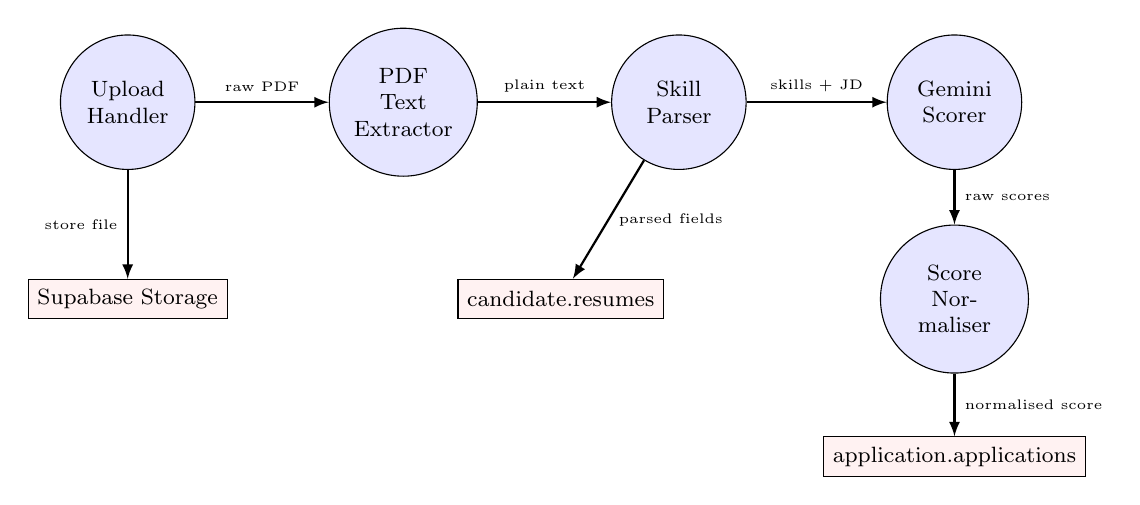
\begin{tikzpicture}[
  process/.style={circle, draw, fill=blue!10, minimum size=1.2cm, font=\footnotesize, text width=1.3cm, align=center},
  store/.style={rectangle, draw, fill=red!5, minimum width=1.8cm, minimum height=0.5cm, font=\footnotesize},
  arrow/.style={-latex, thick, font=\tiny}
]
  \node[process] (p1) at (0,2)   {Upload Handler};
  \node[process] (p2) at (3.5,2) {PDF Text Extractor};
  \node[process] (p3) at (7,2)   {Skill Parser};
  \node[process] (p4) at (10.5,2) {Gemini Scorer};
  \node[process] (p5) at (10.5,-0.5) {Score Normaliser};

  \node[store] (s1) at (0,-0.5) {Supabase Storage};
  \node[store] (s2) at (5.5,-0.5) {candidate.resumes};
  \node[store] (s3) at (10.5,-2.5) {application.applications};

  \draw[arrow] (p1) -- (p2) node[midway, above] {raw PDF};
  \draw[arrow] (p1) -- (s1) node[midway, left] {store file};
  \draw[arrow] (p2) -- (p3) node[midway, above] {plain text};
  \draw[arrow] (p3) -- (s2) node[midway, right] {parsed fields};
  \draw[arrow] (p3) -- (p4) node[midway, above] {skills + JD};
  \draw[arrow] (p4) -- (p5) node[midway, right] {raw scores};
  \draw[arrow] (p5) -- (s3) node[midway, right] {normalised score};
\end{tikzpicture}
}
\caption{DFD Level 2 --- ATS scoring subsystem decomposition}
\label{fig:dfd2}
\end{figure}

The upload handler receives the PDF file from the candidate's browser, validates the file type and size, and stores the original document in Supabase Storage. The PDF text extractor converts the binary PDF into plain text, handling common formatting challenges such as multi-column layouts and header/footer artifacts. The skill parser identifies technical skills, educational qualifications, and experience durations from the extracted text using pattern matching and NLP heuristics. The parsed fields are stored in the \texttt{candidate.resumes} table for future reference.

The Gemini scorer then receives the parsed skills and the job description, constructs a structured evaluation prompt, and sends it to the Gemini API. The API returns dimensional scores (skills match, experience relevance, overall fit) as floating-point values. The score normaliser validates the returned values, clamps them to the 0--10 range, and persists the final composite score in the \texttt{application.applications} table.

\section{Activity Diagram --- Candidate Application Lifecycle}
\label{sec:activity}

Figure~\ref{fig:activity} models the complete lifecycle of a candidate's interaction with SmartHire, from initial registration through to offer acceptance or rejection. Decision points represent system-enforced thresholds that determine whether a candidate advances to the next evaluation stage.

\begin{figure}[htbp]
\centering
\resizebox{0.95\textwidth}{!}{
\begin{tikzpicture}[
  start/.style={circle, draw, fill=black, minimum size=0.3cm},
  stop/.style={circle, draw, fill=black, minimum size=0.3cm, double},
  action/.style={rectangle, draw, rounded corners, fill=green!8, text width=8em, text centered, minimum height=1.8em, font=\small},
  decision/.style={diamond, draw, fill=yellow!12, text width=4.5em, text centered, aspect=2.2, font=\small},
  arrow/.style={-latex, thick}
]
  \node[start]    (s)  at (0,0) {};
  \node[action]   (a1) at (3,0) {Register and Login};
  \node[action]   (a2) at (7,0) {Browse Jobs};
  \node[action]   (a3) at (11,0) {Apply with Resume};
  \node[action]   (a4) at (11,-2) {ATS Score Computed};
  \node[decision] (d1) at (11,-4) {Score $\geq$ threshold?};
  \node[action]   (a5) at (11,-6.5) {Take MCQ Exam};
  \node[decision] (d2) at (11,-8.5) {MCQ pass?};
  \node[action]   (a6) at (11,-10.5) {Solve Coding Challenge};
  \node[decision] (d3) at (11,-12.5) {Code pass?};
  \node[action]   (a7) at (5,-12.5) {AI Video Interview};
  \node[action]   (a8) at (5,-14.5) {Recruiter Reviews};
  \node[action]   (a9) at (5,-16.5) {Offer Extended};
  \node[action]   (rej) at (5,-8.5) {Rejected (stage recorded)};
  \node[stop]     (e)  at (5,-18.5) {};

  \draw[arrow] (s) -- (a1);
  \draw[arrow] (a1) -- (a2);
  \draw[arrow] (a2) -- (a3);
  \draw[arrow] (a3) -- (a4);
  \draw[arrow] (a4) -- (d1);
  \draw[arrow] (d1) -- node[right, font=\footnotesize]{Yes} (a5);
  \draw[arrow] (d1) -| node[above, font=\footnotesize]{No} (rej);
  \draw[arrow] (a5) -- (d2);
  \draw[arrow] (d2) -- node[right, font=\footnotesize]{Yes} (a6);
  \draw[arrow] (d2) -- node[above, font=\footnotesize]{No} (rej);
  \draw[arrow] (a6) -- (d3);
  \draw[arrow] (d3) -- node[above, font=\footnotesize]{Yes} (a7);
  \draw[arrow] (d3) -| node[above, font=\footnotesize]{No} (rej);
  \draw[arrow] (a7) -- (a8);
  \draw[arrow] (a8) -- (a9);
  \draw[arrow] (a9) -- (e);
\end{tikzpicture}
}
\caption{Activity diagram for the candidate application lifecycle}
\label{fig:activity}
\end{figure}

The activity diagram reveals the sequential, gate-keeping nature of SmartHire's evaluation pipeline. Each stage produces a quantitative score, and advancement requires meeting a configurable threshold. This design ensures that only candidates who demonstrate competence at each level proceed to the next, reducing the evaluation burden on later (more expensive) stages such as coding challenges and video interviews. When a candidate is rejected, the specific stage at which the rejection occurred is recorded, enabling the transparent feedback mechanism described in Chapter~1.

\section{Complete SmartHire Recruitment Workflow}
\label{sec:complete-workflow}

This section presents the end-to-end workflow that ties together all system components, from job posting creation by a recruiter to the final hiring decision.

\begin{enumerate}[leftmargin=1.5em]
  \item \textbf{Job Posting}: A recruiter creates a job posting in draft status, specifying the title, description, required skills, location, salary range, and employment type. The recruiter publishes the job when ready, making it visible on the candidate portal.

  \item \textbf{Candidate Application}: A candidate discovers the job listing, reviews the description, and applies by uploading their PDF resume. The system immediately triggers the ATS scoring pipeline.

  \item \textbf{ATS Screening}: The resume text is extracted, parsed, and evaluated against the job requirements via the Gemini API. The resulting score (0--10) is stored with the application. Candidates above the threshold advance; those below receive a rejection notification with their score.

  \item \textbf{MCQ Assessment}: Qualifying candidates are invited to complete a timed MCQ examination. Questions are drawn from the job's question pool and presented in randomised order. The timer enforces auto-submission. Scores are computed and stored instantly.

  \item \textbf{Coding Challenge}: Candidates who pass the MCQ stage are presented with coding problems in the Monaco IDE. They write solutions, run them against sample test cases, and submit for evaluation against the hidden test suite. The percentage of passing tests determines their coding score.

  \item \textbf{AI Video Interview}: Qualifying candidates enter the video interview room, where they respond to structured questions while being recorded. Transcriptions are sent to Gemini for evaluation, producing a detailed scorecard.

  \item \textbf{Recruiter Review}: The recruiter reviews the candidate's complete evaluation profile on the Kanban board: ATS score, MCQ score, coding score, and AI interview scorecard. Based on this data, the recruiter decides to advance, reject, or schedule a follow-up.

  \item \textbf{Offer Generation}: For selected candidates, the recruiter generates a customised PDF offer letter specifying salary, position, joining date, and terms. The offer is sent through the platform.

  \item \textbf{Candidate Response}: The candidate views the offer on their portal and accepts or declines. The response updates the application status and the recruiter's pipeline board.
\end{enumerate}

\section{Module Interaction Matrix}
\label{sec:module-interaction}

Table~\ref{tab:module-matrix} documents the dependencies between SmartHire's principal modules. Each cell indicates whether the row module invokes or depends on the column module during normal operation.

\begin{table}[htbp]
\centering
\caption{Module interaction matrix}
\label{tab:module-matrix}
\small
\begin{tabular}{l|cccccc}
\toprule
 & \rotatebox{60}{\textbf{Auth}} & \rotatebox{60}{\textbf{Job Mgmt}} & \rotatebox{60}{\textbf{ATS}} & \rotatebox{60}{\textbf{Assessment}} & \rotatebox{60}{\textbf{Interview}} & \rotatebox{60}{\textbf{Offer}} \\
\midrule
Auth        & ---          & ---          & ---          & ---          & ---          & ---          \\
Job Mgmt    & \checkmark   & ---          & ---          & ---          & ---          & ---          \\
ATS         & \checkmark   & \checkmark   & ---          & ---          & ---          & ---          \\
Assessment  & \checkmark   & \checkmark   & \checkmark   & ---          & ---          & ---          \\
Interview   & \checkmark   & \checkmark   & ---          & \checkmark   & ---          & ---          \\
Offer       & \checkmark   & \checkmark   & ---          & ---          & ---          & ---          \\
\bottomrule
\end{tabular}
\end{table}

The matrix confirms that the authentication module is a universal dependency, as every operation requires identity verification. The ATS and assessment modules depend on job management for retrieving job specifications and question pools. The interview module depends on the assessment module to verify that the candidate has completed prior stages before being allowed to proceed.

\section{API Request-Response Lifecycle}
\label{sec:api-lifecycle}

Every API request in SmartHire follows a standardised lifecycle through five processing phases:

\begin{enumerate}[leftmargin=1.5em]
  \item \textbf{Authentication}: The middleware extracts the JWT from the request cookie, verifies its signature and expiration using Supabase's \texttt{getUser()} method, and attaches the authenticated user object to the request context. Unauthenticated requests receive a 401 response.

  \item \textbf{Authorisation}: The route handler checks whether the authenticated user has the required role (candidate, recruiter, or admin) for the requested operation. Requests from users with insufficient privileges receive a 403 response.

  \item \textbf{Validation}: Request body parameters are validated against predefined schemas using runtime validation. Malformed requests receive a 400 response with descriptive error messages.

  \item \textbf{Business Logic}: The validated request is processed by the appropriate service module, which may involve database queries, external API calls (Gemini), file operations (Supabase Storage), or a combination thereof.

  \item \textbf{Response}: The result is serialised to JSON and returned with an appropriate HTTP status code (200 for success, 201 for resource creation, 400/401/403/404/500 for various error conditions).
\end{enumerate}

This standardised lifecycle ensures consistent error handling, security enforcement, and response formatting across all endpoints.
